% Template for Cogsci submission with R Markdown

% Stuff changed from original Markdown PLOS Template
\documentclass[10pt, letterpaper]{article}

\usepackage{cogsci}
\usepackage{pslatex}
\usepackage{float}
\usepackage{caption}

% amsmath package, useful for mathematical formulas
\usepackage{amsmath}

% amssymb package, useful for mathematical symbols
\usepackage{amssymb}

% hyperref package, useful for hyperlinks
\usepackage{hyperref}

% graphicx package, useful for including eps and pdf graphics
% include graphics with the command \includegraphics
\usepackage{graphicx}

% Sweave(-like)
\usepackage{fancyvrb}
\DefineVerbatimEnvironment{Sinput}{Verbatim}{fontshape=sl}
\DefineVerbatimEnvironment{Soutput}{Verbatim}{}
\DefineVerbatimEnvironment{Scode}{Verbatim}{fontshape=sl}
\newenvironment{Schunk}{}{}
\DefineVerbatimEnvironment{Code}{Verbatim}{}
\DefineVerbatimEnvironment{CodeInput}{Verbatim}{fontshape=sl}
\DefineVerbatimEnvironment{CodeOutput}{Verbatim}{}
\newenvironment{CodeChunk}{}{}

% cite package, to clean up citations in the main text. Do not remove.
\usepackage{apacite}

% KM added 1/4/18 to allow control of blind submission
\cogscifinalcopy

\usepackage{color}

% Use doublespacing - comment out for single spacing
%\usepackage{setspace}
%\doublespacing


% % Text layout
% \topmargin 0.0cm
% \oddsidemargin 0.5cm
% \evensidemargin 0.5cm
% \textwidth 16cm
% \textheight 21cm

\title{When \emph{doggy} becomes \emph{dog}: Developmental shifts the
use of register-specific words}

\usepackage{booktabs}
\usepackage{longtable}
\usepackage{array}
\usepackage{multirow}
\usepackage{wrapfig}
\usepackage{float}
\usepackage{colortbl}
\usepackage{pdflscape}
\usepackage{tabu}
\usepackage{threeparttable}
\usepackage{threeparttablex}
\usepackage[normalem]{ulem}
\usepackage{makecell}
\usepackage{xcolor}

\author{{\large \bf Kennedy Casey} \\ University of Chicago \\ \texttt{kbcasey@uchicago.edu} \And {\large \bf Marisa Casillas} \\ University of Chicago \\ \texttt{mcasillas@uchicago.edu}}

\newlength{\cslhangindent}
\setlength{\cslhangindent}{1.5em}
\newenvironment{CSLReferences}%
  {}%
  {\par}

\begin{document}

\maketitle

\begin{abstract}
Child-directed speech (CDS) features words such as \emph{doggy},
\emph{night-night}, and \emph{tummy} that are rarely used in
adult-directed speech (ADS). Characterisitcs of CDS word forms, such as
reduplication and diminutivization, explain why they may be learned and
produced earlier by children. However, it is not yet clear how or when
children switch to using ADS equivalents---\emph{dog}, \emph{goodnight},
\emph{stomach}. Through analysis of transcripts from CHILDES and the
Language Development Project corpus, we show that children significantly
increase their production of ADS word forms across age, with the average
CDS-to-ADS transition point at 2.5 years. Many of the linguistic
features that distinguish CDS vs.~ADS registers (e.g., speech rate,
lexical complexity, etc.) similarly differentiated the local speech
contexts surrounding CDS vs.~ADS word forms. Learners may therefore be
able to capitalize on these cues to support their discovery of register
and context-appropriate CDS/ADS pair use.

\textbf{Keywords:}
child-directed speech; word production; linguistic input; social
register; corpus analysis; developmental change
\end{abstract}

\hypertarget{introduction}{%
\section{Introduction}\label{introduction}}

Across many cultures and languages, speech that is addressed to children
sounds remarkably different from speech that is addressed to adults
(REFS). When communicating with young children, adults often modify
their speech in ways that draw children's attention and support their
several aspects of their language learning (e.g., Nencheva, Piazza, \&
Lew-Williams, 2021; Rowe, 2008; Shneidman \& Goldin-Meadow, 2012;
Weisleder \& Fernald, 2013).

\hypertarget{child-directed-speech-as-a-simplified-register}{%
\subsection{Child-directed speech as a simplified
register}\label{child-directed-speech-as-a-simplified-register}}

Very brief description of some modifications to CDS (foreshadowing later
in-depth look at prosodic, lexical, and syntactic features in Study 2
input analyses). In broad strokes, the general idea is that CDS is
simpler and tailored such that it helps young learners. However, some
modifications to CDS seem to complicate learning.

\hypertarget{register-specific-words-in-early-vocabulary}{%
\subsection{Register-specific words in early
vocabulary}\label{register-specific-words-in-early-vocabulary}}

Of interest here is the inclusion of register-specific words, such as
\emph{doggy}, \emph{night-night}, and \emph{tummy}, that have
straightforward ADS equivalents (hereafter, `CDS forms' vs.~`ADS forms.'
Why have two labels when one is sufficient for communication? Add ref to
EC principle of contrast. Add some refs to ME work, establishing the
idea that kids generally expect one-to-one form-meaning mappings.

Review of previous research focusing on the learnability question or why
these words appear in the first place. Diminutive suffix as a decently
reliable cue to word ending (\textbf{kempe2005diminutives?}).
Diminutivization and reduplication predictive of vocabulary growth
(\textbf{ota2018choo?}).

Existing research does well to account for why CDS forms make up a large
proportion of the input and why they are learned and produced earlier by
children. However, a later step in vocabulary development requires
children to shift away from using CDS forms in favor of conventionalized
ADS forms. That is, at some point, the animal that was frequently called
\emph{doggy} almost exclusively becomes \emph{dog}.

\hypertarget{current-investigation}{%
\subsection{Current investigation}\label{current-investigation}}

Somewhat oversimplified view of vocabulary development in the field.
Focus on binary (often caregiver-reported) measures of when children
`know' a word's meaning. For good reason, vocabulary questionnaires,
including the standard MacArthur-Bates Communicative Development
Inventory (Fenson et al., 1994), gloss over variations in form. This
helps with generalizing over idiosyncratic words and developing
articulation skills but misses the opportunity to investigate meaningful
shifts in form across time.

In Study 1, we analyze existing speech corpora for children up to seven
years of age to determine if and when we can detect a shift from
production of CDS forms to ADS forms. After establishing that a shift
toward production of ADS forms occurs in early childhood, we explore, in
Study 2, what information in children's linguistic input could support
this shift.

\hypertarget{study-1-when-do-children-shift-from-cds-to-ads-forms}{%
\section{Study 1: When do children shift from CDS to ADS
forms?}\label{study-1-when-do-children-shift-from-cds-to-ads-forms}}

We tracked children's usage of 15 CDS/ADS word pairs (Table
\ref{tab:tab1}) from infancy up to age seven. Since CDS forms rarely
appear in ADS, we predicted that children shift away from production of
these register-specific forms with increasing age. That is, we expected
to see replacement of CDS forms with ADS forms in children's own speech
across time.

\hypertarget{method}{%
\section{Method}\label{method}}

\hypertarget{corpora}{%
\subsection{Corpora}\label{corpora}}

We analyzed 8251 transcripts in the North American English collection of
the Child Language Data Exchange System (CHILDES) database (MacWhinney,
2000) for children up to 7 years of age. The included transcripts were
drawn from 52 individual corpora and featured 980 children (age range =
1--84 months, \emph{M} = 33.5 months). Child production data from the
Language Development Project (LDP) longitudinal corpus were also
analyzed (see Rowe, 2008; \textbf{huttenlocher2010sources?} for further
details regarding participating families, recording procedures, and
transcription). These included 622 transcripts from 59 English-learning
children recorded every 4 months for approximately 90 minutes from age
14 to 58 months.

\hypertarget{target-words}{%
\subsection{Target words}\label{target-words}}

Fifteen CDS/ADS word pairs (30 total target words) were selected based
on two criteria: the appearance of at least one form on the CDI (Fenson
et al., 1994), and sufficient frequency of occurrence in CHILDES (at
least 100 child-produced tokens and 100 other-produced tokens per form).
Pairs were also selected based on researcher intuition to ensure that
that the same object, animal, or routine could be reasonably labeled
with either form (e.g., \emph{doggy} or \emph{dog}) by children.

\begin{table}[ht]
\centering
\resizebox{\linewidth}{!}{
\begin{tabular}{rlrrrr}
  \toprule
\multicolumn{2}{c}{\textbf{ }} & \multicolumn{2}{c}{\textbf{CDS tokens by speaker}} & \multicolumn{2}{c}{\textbf{ADS tokens by speaker}} \\
\cmidrule(l{3pt}r{3pt}){3-4} \cmidrule(l{3pt}r{3pt}){5-6}
\textbf{} & \textbf{Pair} & \textbf{Child} & \textbf{Other} & \textbf{Child} & \textbf{Other }\\ 
  \midrule
1 & doggy/dog & 2249 & 2644 & 3519 & 5113 \\ 
  2 & kitty/cat & 1552 & 3309 & 2779 & 4443 \\ 
  3 & tummy/stomach & 435 & 623 & 112 & 360 \\ 
  4 & daddy/dad & 9603 & 10048 & 2313 & 1031 \\ 
  5 & mommy/mom & 20294 & 17070 & 7616 & 2552 \\ 
  6 & bunny/rabbit & 1237 & 2597 & 1060 & 1397 \\ 
  7 & duckie/duck & 307 & 647 & 1933 & 3003 \\ 
  8 & blankie/blanket & 174 & 224 & 825 & 874 \\ 
  9 & froggy/frog & 154 & 434 & 970 & 1846 \\ 
  10 & potty/bathroom & 511 & 786 & 161 & 270 \\ 
  11 & night night/goodnight & 149 & 153 & 102 & 446 \\ 
  12 & dolly/doll & 745 & 1054 & 674 & 2697 \\ 
  13 & horsey/horse & 1149 & 1034 & 1749 & 2575 \\ 
  14 & piggy/pig & 405 & 1212 & 1276 & 2139 \\ 
  15 & birdie/bird & 399 & 588 & 1879 & 3358 \\ 
   \bottomrule
\end{tabular}}
\caption{CHILDES frequency for 15 CDS/ADS word pairs. Child-produced
                             counts include tokens produced only by the target child.} 
\label{tab:tab1}
\end{table}

\hypertarget{results}{%
\section{Results}\label{results}}

We first asked when CDS forms are replaced by ADS forms in children's
own speech. We fit a mixed-effects binomial logistic regression model
predicting children's production of CDS vs.~ADS forms, with target child
age (in months, scaled) as a single fixed effect. Random slopes and
intercepts for word pairs were also included. For each target word
token, the form was coded as either 0 (CDS) or 1 (ADS). Thus, the model
captures, for each age, the relative proportion of CDS vs.~ADS forms in
children's own speech.

Children's production of ADS forms increased with age (\(\beta\) = 0.54,
\emph{SE} = 0.11, \emph{t} = 4.92, \emph{p} \textless{} 0.001). This
trend of increasing ADS form production was significant for 13 of 15
pairs. The average CDS-to-ADS transition point (i.e., the point at which
ADS forms were produced \textgreater50\% of the time) was between 24 and
36 months of age (Figure 1).

\begin{CodeChunk}
\begin{figure}[h]

{\centering 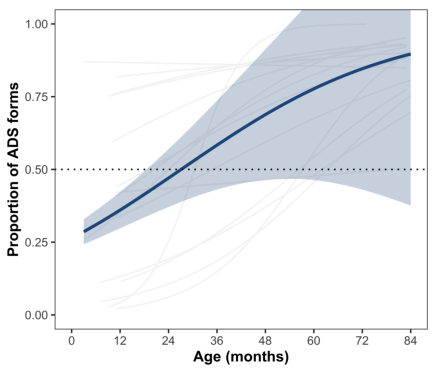
\includegraphics{figs/shift-timing-fig-1} 

}

\caption[Model-predicted increase in production of ADS forms with age]{Model-predicted increase in production of ADS forms with age. Gray lines depict individual word-pair trajectories.}\label{fig:shift-timing-fig}
\end{figure}
\end{CodeChunk}

\begin{CodeChunk}
\begin{figure*}[!ht]

{\centering 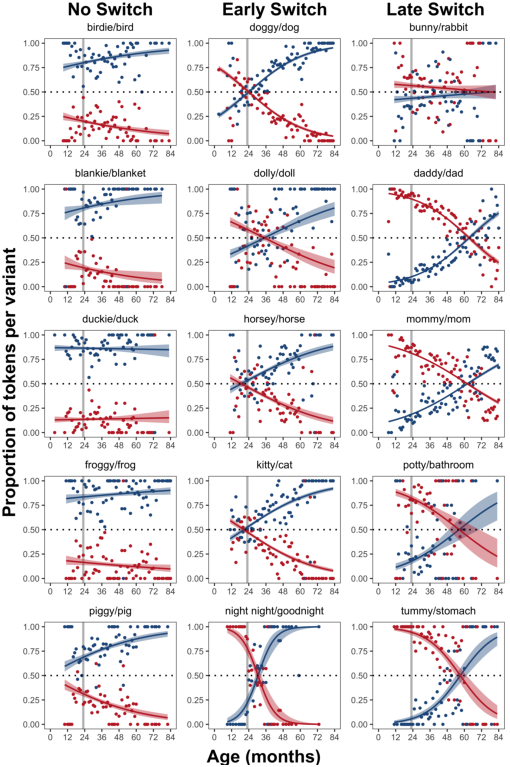
\includegraphics{figs/shift-timing-bypair-fig-1} 

}

\caption[Inidividual word-pair trajectories for increasing production of ADS forms (blue) and descreasing production of CDS forms (red) with age]{Inidividual word-pair trajectories for increasing production of ADS forms (blue) and descreasing production of CDS forms (red) with age. Points indicate proportions for each 1-month age bin.}\label{fig:shift-timing-bypair-fig}
\end{figure*}
\end{CodeChunk}

\hypertarget{study-2-what-linguisitc-information-in-childrens-input-supports-their-shift-from-cds-to-ads-forms}{%
\section{Study 2: What linguisitc information in children's input
supports their shift from CDS to ADS
forms?}\label{study-2-what-linguisitc-information-in-childrens-input-supports-their-shift-from-cds-to-ads-forms}}

\begin{CodeChunk}
\begin{figure*}[h]

{\centering 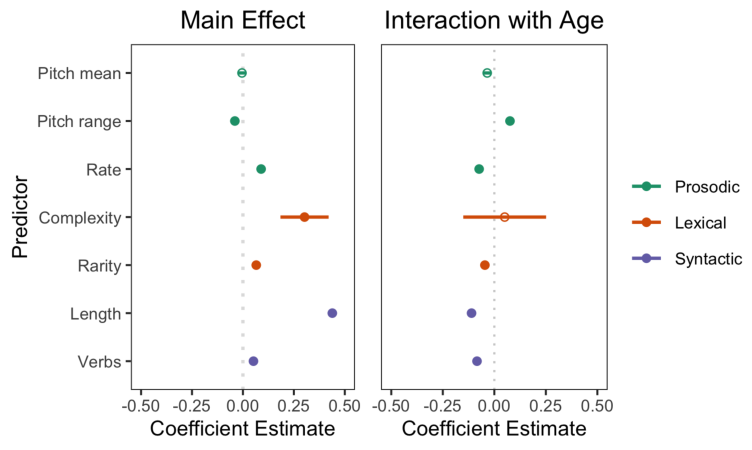
\includegraphics{figs/model-plot-1} 

}

\caption[Coefficient estimates for linguistic predictors of form]{Coefficient estimates for linguistic predictors of form. Positive main effects indicate that utterances are more likely to contain ADS forms when they have higher values for the predictor (e.g., faster speech rates). Positive age interactions indicate an increasing effect of the predictor with age. Error bars depict standard errors of the coefficient estimates, and filled circles represent significant effects (\textit{p} $<$ 0.05).}\label{fig:model-plot}
\end{figure*}
\end{CodeChunk}

We next explored children's input (i.e., other-produced speech), asking
whether the linguistic features that differentiate CDS vs.~ADS at the
register level also differentiate the local speech contexts surrounding
CDS vs.~ADS forms. In other words, can form be predicted on the basis of
individual utterance-level prosodic, lexical, or syntactic cues?

\hypertarget{method-1}{%
\section{Method}\label{method-1}}

\hypertarget{corpora-1}{%
\subsection{Corpora}\label{corpora-1}}

Reference above but drop LDP

\hypertarget{linguistic-input-predictors}{%
\subsection{Linguistic input
predictors}\label{linguistic-input-predictors}}

All input analyses were conducted over individual other-produced
utterances in CHILDES (i.e., speech not produced by the target child).
We quantified prosodic, lexical, and syntactic information to describe
each utterance containing one of the 30 target words.

\hypertarget{prosodic-level}{%
\subsubsection{Prosodic level}\label{prosodic-level}}

We measured three types of prosodic information: \textbf{mean pitch}
(Hz), \textbf{pitch range} (Hz), and \textbf{speech rate} (words per
second). These measures were calculated over all timestamped utterances
in CHILDES (42.3\% of other-produced utterances). Utterances shorter
than 58 ms were excluded from analysis. This lower bound was set by
identifying the the shortest possible duration of an utterance
containing at least one word in four manually annotated North American
English corpora in HomeBank (Bergelson, 2016; McDivitt \& Soderstrom,
2016; VanDam et al., 2016; VanDam, 2016; Warlaumont \& Pretzer, 2016) .
Pitch information was extracted using Praat software (Boersma \&
Weenink, 2016).

\hypertarget{lexical-level}{%
\subsubsection{Lexical level}\label{lexical-level}}

We measured two types of lexical information: complexity and rarity.
\textbf{Lexical complexity} was defined as the negative log proportion
of known words in each utterance (consistent with Foushee, Griffiths, \&
Srinivasan, 2016; Kidd, Piantadosi, \& Aslin, 2012). A word was
considered `known' if the age of acquisition (AoA) estimate (Fenson et
al., 1994; Frank, Braginsky, Yurovsky, \& Marchman, 2017) was less than
or equal to the age of the target child when they heard the utterance.
Utterances with proportionally fewer known words are more lexically
complex. \textbf{Lexical rarity} was determined based on overall
frequency in CHILDES. For all words with at least 10 tokens\footnote{Manual
  checks revealed that many of the lowest-frequency words included
  idiosyncratic or erroneous transcriptions and/or repetitions of
  non-words from children's babbling.}, we calculated a rarity score as
the negative log proportion of other-produced tokens in CHILDES (i.e.,
number of tokens for a given word/sum of all tokens in the full corpus),
and then averaged for rarity scores for all target utterances.
Utterances with more low-frequency words are considered more lexically
rare.

\hypertarget{syntactic-level}{%
\subsubsection{Syntactic level}\label{syntactic-level}}

Syntactic measures included both the utterance \textbf{length} (in
words) and \textbf{number of verb phrases}. The number of words per
utterance was automatically extracted using the \texttt{childesr}
package (Braginsky, Sanchez, \& Yurovsky, 2021). The number of verb
phrases per utterance was determined using \texttt{spaCy3}, an automatic
syntactic parser (Honnibal, Montani, Van Landeghem, \& Boyd, 2020).

\hypertarget{results-1}{%
\section{Results}\label{results-1}}

We ran individual mixed-effects binomial logistic regression models for
each of seven linguisitc input predictors. Models included fixed effects
of linguistic predictor, target child age, and their interaction as well
as random intercepts for individual word pairs and speakers. For each
target word token, form was coded as CDS (0) or ADS (1), so coefficient
estimates should be interpreted as an indication of the likelihood that
an utterance contains an ADS form. All main effects of linguistic
predictors and interactions with age are shown in Figure 3.

At the prosodic level, we found significant effects for two of three
input predictors tested. Utterance-level \textbf{pitch range} was not
predictive of form (\(\beta\) = 0.002, \emph{SE} = 0.02, \emph{t} = 0.1,
\emph{p} = 0.919) and did not significantly interact with age (\(\beta\)
= 0.02, \emph{SE} = 0.02, \emph{t} = 1.11, \emph{p} = 0.268). However,
utterance-level \textbf{mean pitch} was a negative predictor of ADS form
(\(\beta\) = -0.058, \emph{SE} = 0.02, \emph{t} = -3.02, \emph{p} =
0.003). That is, utterances with higher overall mean pitch were more
likely to contain CDS forms, with so significant interaction with age
(\(\beta\) = -0.02, \emph{SE} = 0.02, \emph{t} = -0.96, \emph{p} =
0.337). \textbf{Speech rate} (i.e., words produced per second) was a
positive predictor of ADS form (\(\beta\) = 0.09, \emph{SE} = 0.02,
\emph{t} = 4.86, \emph{p} \textless{} 0.001). Utterances spoken more
quickly were more likely to contain ADS forms. This input predictor also
negatively interacted with age (\(\beta\) = -0.07, \emph{SE} = 0.02,
\emph{t} = -3.96, \emph{p} \textless{} 0.001), indicating a decreasing
strength in predictive power across developmental time.

At the lexical level, we found significant effects for both input
predictors tested. Utterances with higher levels of \textbf{lexical
complexity} (\(\beta\) = 0.27, \emph{SE} = 0.08, \emph{t} = 3.28,
\emph{p} = 0.001) and \textbf{lexical rarity} (\(\beta\) = 0.07,
\emph{SE} = 0.01, \emph{t} = 5.73, \emph{p} \textless{} 0.001) were more
likely to contain ADS forms. Lexical complexity did not interact with
age (\(\beta\) = -0.1, \emph{SE} = 0.21, \emph{t} = -0.47, \emph{p} =
0.637); whereas, lexical rarity negatively interacted with age such that
there was a decreasing effect of this predictor with age (\(\beta\) =
-0.05, \emph{SE} = 0.01, \emph{t} = -3.95, \emph{p} \textless{} 0.001).

At the syntactic level, we found significant effects of
\textbf{utterance length} and \textbf{number of verb phrases}.
Utterances with more words (\(\beta\) = 0.19, \emph{SE} = 0.01, \emph{t}
= 16.3, \emph{p} \textless{} 0.001) and more verb phrases (\(\beta\) =
0.05, \emph{SE} = 0.01, \emph{t} = 4.44, \emph{p} \textless{} 0.001)
were more likely to contain ADS forms. Moreover, both linguistic
predictors negatively interacted with age (Length: \(\beta\) = -0.16,
\emph{SE} = 0.01, \emph{t} = -14.61, \emph{p} \textless{} 0.001; Verbs:
\(\beta\) = -0.08, \emph{SE} = 0.01, \emph{t} = -7.7, \emph{p}
\textless{} 0.001), suggesting that the strength of these predictors
decreases across developmental time.

\hypertarget{discussion}{%
\section{Discussion}\label{discussion}}

\hypertarget{general-discussion}{%
\section{General Discussion}\label{general-discussion}}

\hypertarget{references}{%
\section{References}\label{references}}

\setlength{\parindent}{-0.1in} 
\setlength{\leftskip}{0.125in}

\noindent

\hypertarget{refs}{}
\begin{CSLReferences}{1}{0}
\leavevmode\hypertarget{ref-bergelsoncorpus}{}%
Bergelson, E. (2016). Bergelson HomeBank corpus.
\url{https://doi.org/10.21415/T5PK6D}.

\leavevmode\hypertarget{ref-boersma2016praat}{}%
Boersma, P., \& Weenink, D. (2016). Praat software. \emph{Amsterdam:
University of Amsterdam}.

\leavevmode\hypertarget{ref-braginsky2021childesr}{}%
Braginsky, M., Sanchez, A., \& Yurovsky, D. (2021). \emph{Childesr:
Accessing the 'CHILDES' database}. Retrieved from
\url{https://CRAN.R-project.org/package=childesr}

\leavevmode\hypertarget{ref-fenson1994variability}{}%
Fenson, L., Dale, P. S., Reznick, J. S., Bates, E., Thal, D. J.,
Pethick, S. J., \ldots{} Stiles, J. (1994). Variability in early
communicative development. \emph{Monographs of the Society for Research
in Child Development}, i--185.

\leavevmode\hypertarget{ref-foushee2016lexical}{}%
Foushee, R., Griffiths, T., \& Srinivasan, M. (2016). Lexical complexity
of child-directed and overheard speech: Implications for learning. In
\emph{Proceedings of the 38th annual conference of the cognitive science
society} (pp. 1697--1702).

\leavevmode\hypertarget{ref-frank2017wordbank}{}%
Frank, M. C., Braginsky, M., Yurovsky, D., \& Marchman, V. A. (2017).
Wordbank: An open repository for developmental vocabulary data.
\emph{Journal of Child Language}, \emph{44}(3), 677--694.

\leavevmode\hypertarget{ref-honnibal2020spacy}{}%
Honnibal, M., Montani, I., Van Landeghem, S., \& Boyd, A. (2020).
{spaCy: Industrial-strength Natural Language Processing in Python}.
http://doi.org/\href{https://doi.org/10.5281/zenodo.1212303}{10.5281/zenodo.1212303}

\leavevmode\hypertarget{ref-kidd2012goldilocks}{}%
Kidd, C., Piantadosi, S. T., \& Aslin, R. N. (2012). The goldilocks
effect: Human infants allocate attention to visual sequences that are
neither too simple nor too complex. \emph{PloS One}, \emph{7}(5),
e36399.

\leavevmode\hypertarget{ref-macwhinney2000childes}{}%
MacWhinney, B. (2000). \emph{The CHILDES project: The database} (Vol.
2). Psychology Press.

\leavevmode\hypertarget{ref-soderstromcorpus}{}%
McDivitt, K., \& Soderstrom, M. (2016). McDivitt HomeBank corpus.
\url{https://doi.org/10.21415/T5KK6G}.

\leavevmode\hypertarget{ref-nencheva2021moment}{}%
Nencheva, M. L., Piazza, E. A., \& Lew-Williams, C. (2021). The
moment-to-moment pitch dynamics of child-directed speech shape toddlers'
attention and learning. \emph{Developmental Science}, \emph{24}(1),
e12997.

\leavevmode\hypertarget{ref-rowe2008child}{}%
Rowe, M. L. (2008). Child-directed speech: Relation to socioeconomic
status, knowledge of child development and child vocabulary skill.
\emph{Journal of Child Language}, \emph{35}(1), 185--205.

\leavevmode\hypertarget{ref-shneidman2012language}{}%
Shneidman, L. A., \& Goldin-Meadow, S. (2012). Language input and
acquisition in a mayan village: How important is directed speech?
\emph{Developmental Science}, \emph{15}(5), 659--673.

\leavevmode\hypertarget{ref-vandamcorpus}{}%
VanDam, M. (2016). VanDam2 HomeBank corpus.

\leavevmode\hypertarget{ref-homebank}{}%
VanDam, M., Warlaumont, A. S., Bergelson, E., Cristia, A., De Palma, P.,
\& MacWhinney, B. (2016). Homebank: An online repository of daylong
child-centered audio recordings. \url{https://homebank.talkbank.org}.

\leavevmode\hypertarget{ref-warlaumontcorpus}{}%
Warlaumont, A. S., \& Pretzer, G. M. (2016). Warlaumont HomeBank corpus.
\url{https://doi.org/10.21415/t54s3c}.

\leavevmode\hypertarget{ref-weisleder2013talking}{}%
Weisleder, A., \& Fernald, A. (2013). Talking to children matters: Early
language experience strengthens processing and builds vocabulary.
\emph{Psychological Science}, \emph{24}(11), 2143--2152.

\end{CSLReferences}

\bibliographystyle{apacite}


\end{document}
